% Validation of a finite-element solver for the one-dimensional retraction of a
% viscous sheet, against an independent implementation and against published
% asymptotics.
%
% Build:  latexmk -pdf validation-1d.tex
\documentclass[11pt,a4paper]{article}

\usepackage[margin=2.4cm]{geometry}
\usepackage{amsmath,amssymb}
\usepackage{graphicx}
\usepackage{booktabs}
\usepackage[hidelinks]{hyperref}
\usepackage{caption}

\newcommand{\TC}{\textsf{TC1D-FEM}}
\newcommand{\AB}{\textsf{ABDS-CN}}
\newcommand{\Xc}{X_{c}}
\newcommand{\Tc}{T_{c}}

\title{Validation of a finite-element solver for one-dimensional viscous sheet
retraction}
\author{CoMPhy Lab}
\date{\today}

\begin{document}
\maketitle

\begin{abstract}
We validate a finite-element solver for the one-dimensional (long-wave)
retraction of a viscous liquid sheet against an independent finite-difference
implementation and against the asymptotic results of Ahsan \textit{et al.}
(arXiv:2507.04603). The two solvers share no code, no discretisation and no
coordinate system, and agree to between $2\times 10^{-5}$ and $1.3\times 10^{-4}$ in the
retraction speed across four decades of time. Measured against the published
asymptotics, the early-time law and the late-time finite-sheet law are
reproduced without adjustable constants, as are the tip-thickness relation and
the crossover time $\Tc = \mathcal{L}$. In the late-time infinite-sheet regime
we find that the speed deficit is well described by
$1 - \mathrm{d}\Xc/\mathrm{d}T \simeq \tfrac{3}{2}(1+T)^{-2}$, where the
published coefficient is unity; the coefficient is stated in that work to be a
numerical fit rather than a result of the asymptotic analysis.
\end{abstract}

\section{Scope and nomenclature}

Two solvers are compared throughout.

\textbf{\TC} is the solver under validation: a finite-element discretisation of
the long-wave equations in a Lagrangian mass coordinate, with the sheet
thickness $h$ on a cell-constant space and the velocity $u$ on continuous
piecewise-linear elements, integrated with BDF2. The free edge is a material
point of the mesh, so no interface tracking or remeshing is required.

\textbf{\AB} is an independent reference: a transcription into Python of the
finite-difference solver released with Ahsan \textit{et al.}, which advances a
Crank--Nicolson discretisation on a static grid with Picard iteration and a
tridiagonal solve. Appendix~\ref{sec:port} establishes that the transcription
reproduces the original code to the precision at which the original can be
read.

The asymptotic predictions of Ahsan \textit{et al.} are treated here as
hypotheses to be tested, and are plotted as such: they are not used to
normalise or calibrate either solver.

\subsection{Units}

Ahsan \textit{et al.} scale on the half-thickness $h_0 = H/2$, with
$u_{TC} = \sqrt{\gamma/\rho h_0}$, Ohnesorge number
$Oh_{p} = \mu/\sqrt{\rho h_0 \gamma}$ and visco-inertial time
$t_I = 4\mu h_0/\gamma$. This work scales on the full thickness $H$, with the
Savva--Bush Ohnesorge number $Oh$ and viscous time
$\tau_{\mathrm{vis}} = \mu H/2\gamma$. The maps are
%
\begin{equation}
  Oh_{p} = 2\,Oh, \qquad T = t^{*}/4, \qquad
  \mathcal{L} = \frac{\ell_0}{4 h_0 Oh_{p}} = \frac{M}{4\,Oh},
  \label{eq:units}
\end{equation}
%
where $t^{*} = t/\tau_{\mathrm{vis}}$ and $M$ is the total sheet mass per unit
width, which is the extent of the computational domain in the mass coordinate.
Their retraction speed $\mathrm{d}\Xc/\mathrm{d}T$ equals $u^{*} = U/V_{TC}$
with no intervening factor. These relations were verified symbolically, and
independently confirmed by two physical identities: their tip condition
$H V_X = -1$ is the natural boundary condition of the present formulation, and
their $H(\Xc,T) = 1+T$ is the tip-thickness relation measured here as
$h_{\mathrm{tip}} = 1 + t^{*}/4$.

Equation~\eqref{eq:units} also shows that the present formulation represents a
sheet of finite length: $\mathcal{L}$ is set by the mass domain $M$, and the
far boundary condition (vanishing velocity, free thickness) is the condition
imposed in the reference work. The mapping was checked before use: at
$M = 20$, $Oh = 1$, the deceleration is observed at $\Tc = 4.97$ against
$\mathcal{L} = 5$.

\section{Early time: \texorpdfstring{$T \ll 1$}{T << 1}}
\label{sec:early}

At early times the reference work predicts a diffusive growth of the retraction
speed, $\mathrm{d}\Xc/\mathrm{d}T \sim 2\sqrt{T/\pi}$ (their eq.~5.10).
Figure~\ref{fig:early} compares both solvers and that prediction at
$\mathcal{L} = 0.1$, $1$ and $20$.

\begin{figure}[htbp]
  \centering
  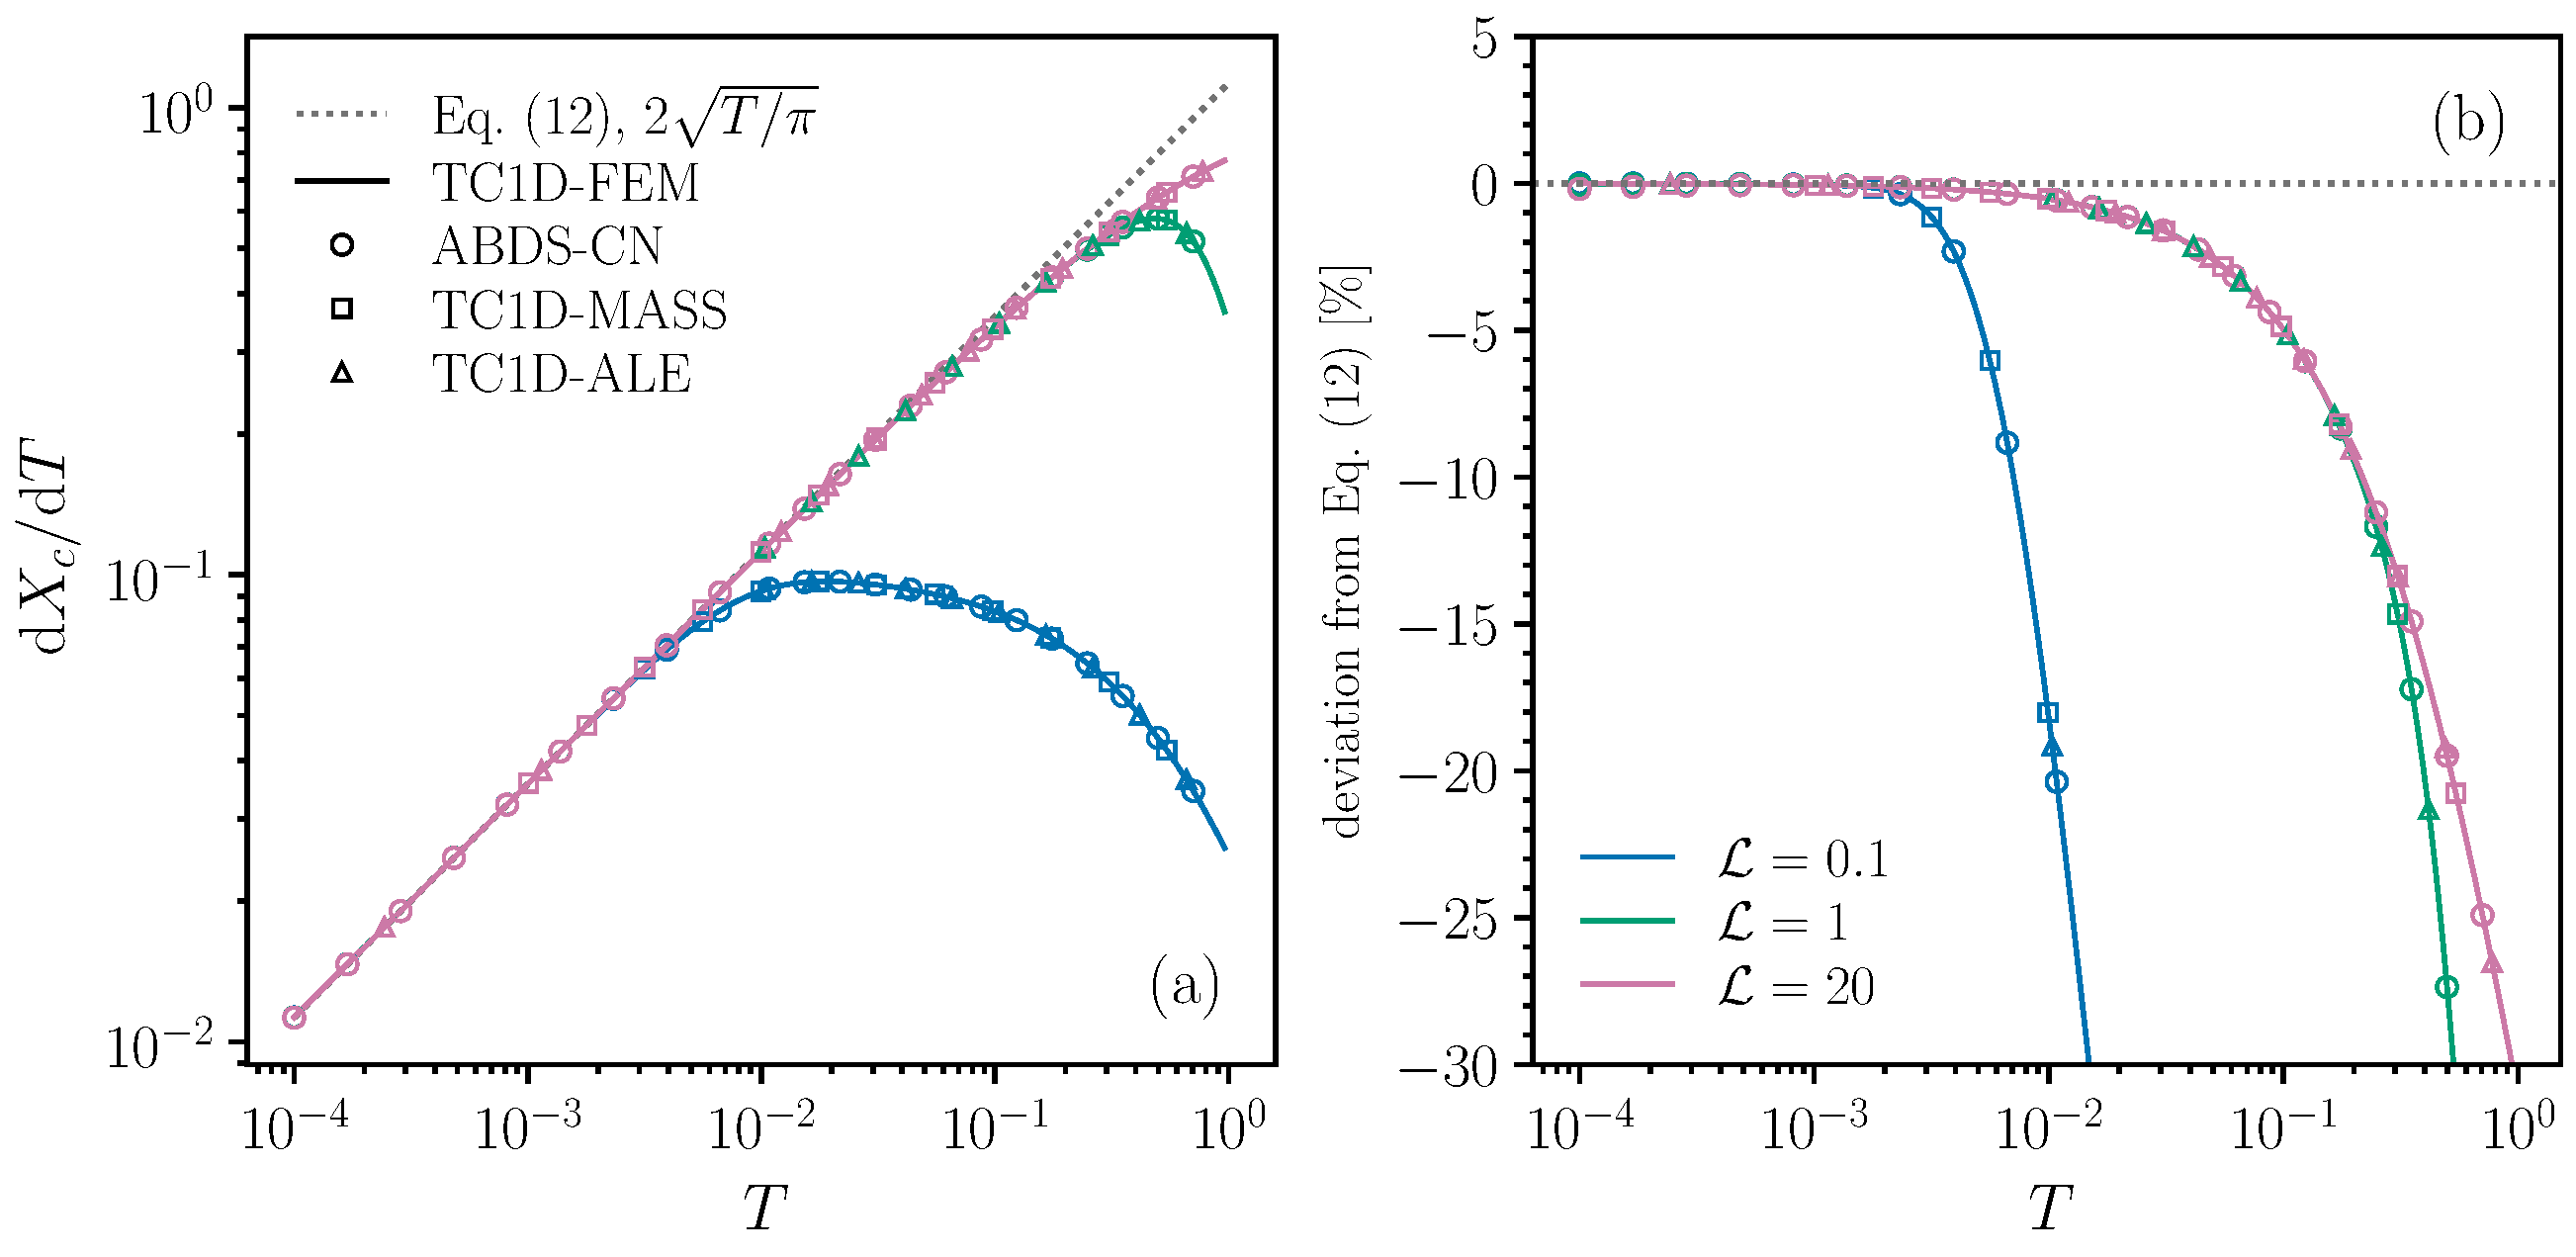
\includegraphics[width=\textwidth]{figures/fig1_earlytime.pdf}
  \caption{Retraction speed at early time. Solid: \TC. Open symbols: \AB.
  Dotted: the diffusive prediction $2\sqrt{T/\pi}$.}
  \label{fig:early}
\end{figure}

The prediction is reproduced to better than 0.06\% for
$T \le 10^{-3}$ at every $\mathcal{L}$. Its range of validity depends strongly
on $\mathcal{L}$: taking the time at which the relative deviation first exceeds
1\%, 5\% and 10\%,

\begin{center}
\begin{tabular}{lccc}
\toprule
 & 1\% & 5\% & 10\% \\
\midrule
$\mathcal{L} = 0.1$ & $T = 0.0031$ & $0.0053$ & $0.0075$ \\
$\mathcal{L} = 1$   & $T = 0.019$  & $0.102$  & $0.213$  \\
\bottomrule
\end{tabular}
\end{center}

The two solvers agree over this window to a maximum absolute difference of
$2.4\times 10^{-5}$ at $\mathcal{L}=0.1$ and $1.3\times 10^{-4}$ at $\mathcal{L}=1$.

\section{Late time at finite length: the deceleration}
\label{sec:decel}

When the free edge approaches the far end of the sheet, $\mathcal{L} - \Xc \ll 1$,
the reference work predicts $\mathrm{d}\Xc/\mathrm{d}T \sim \mathcal{L}(1+T)^{-2}$
(their eq.~6.10). This regime is the principal focus of that work.

\begin{figure}[htbp]
  \centering
  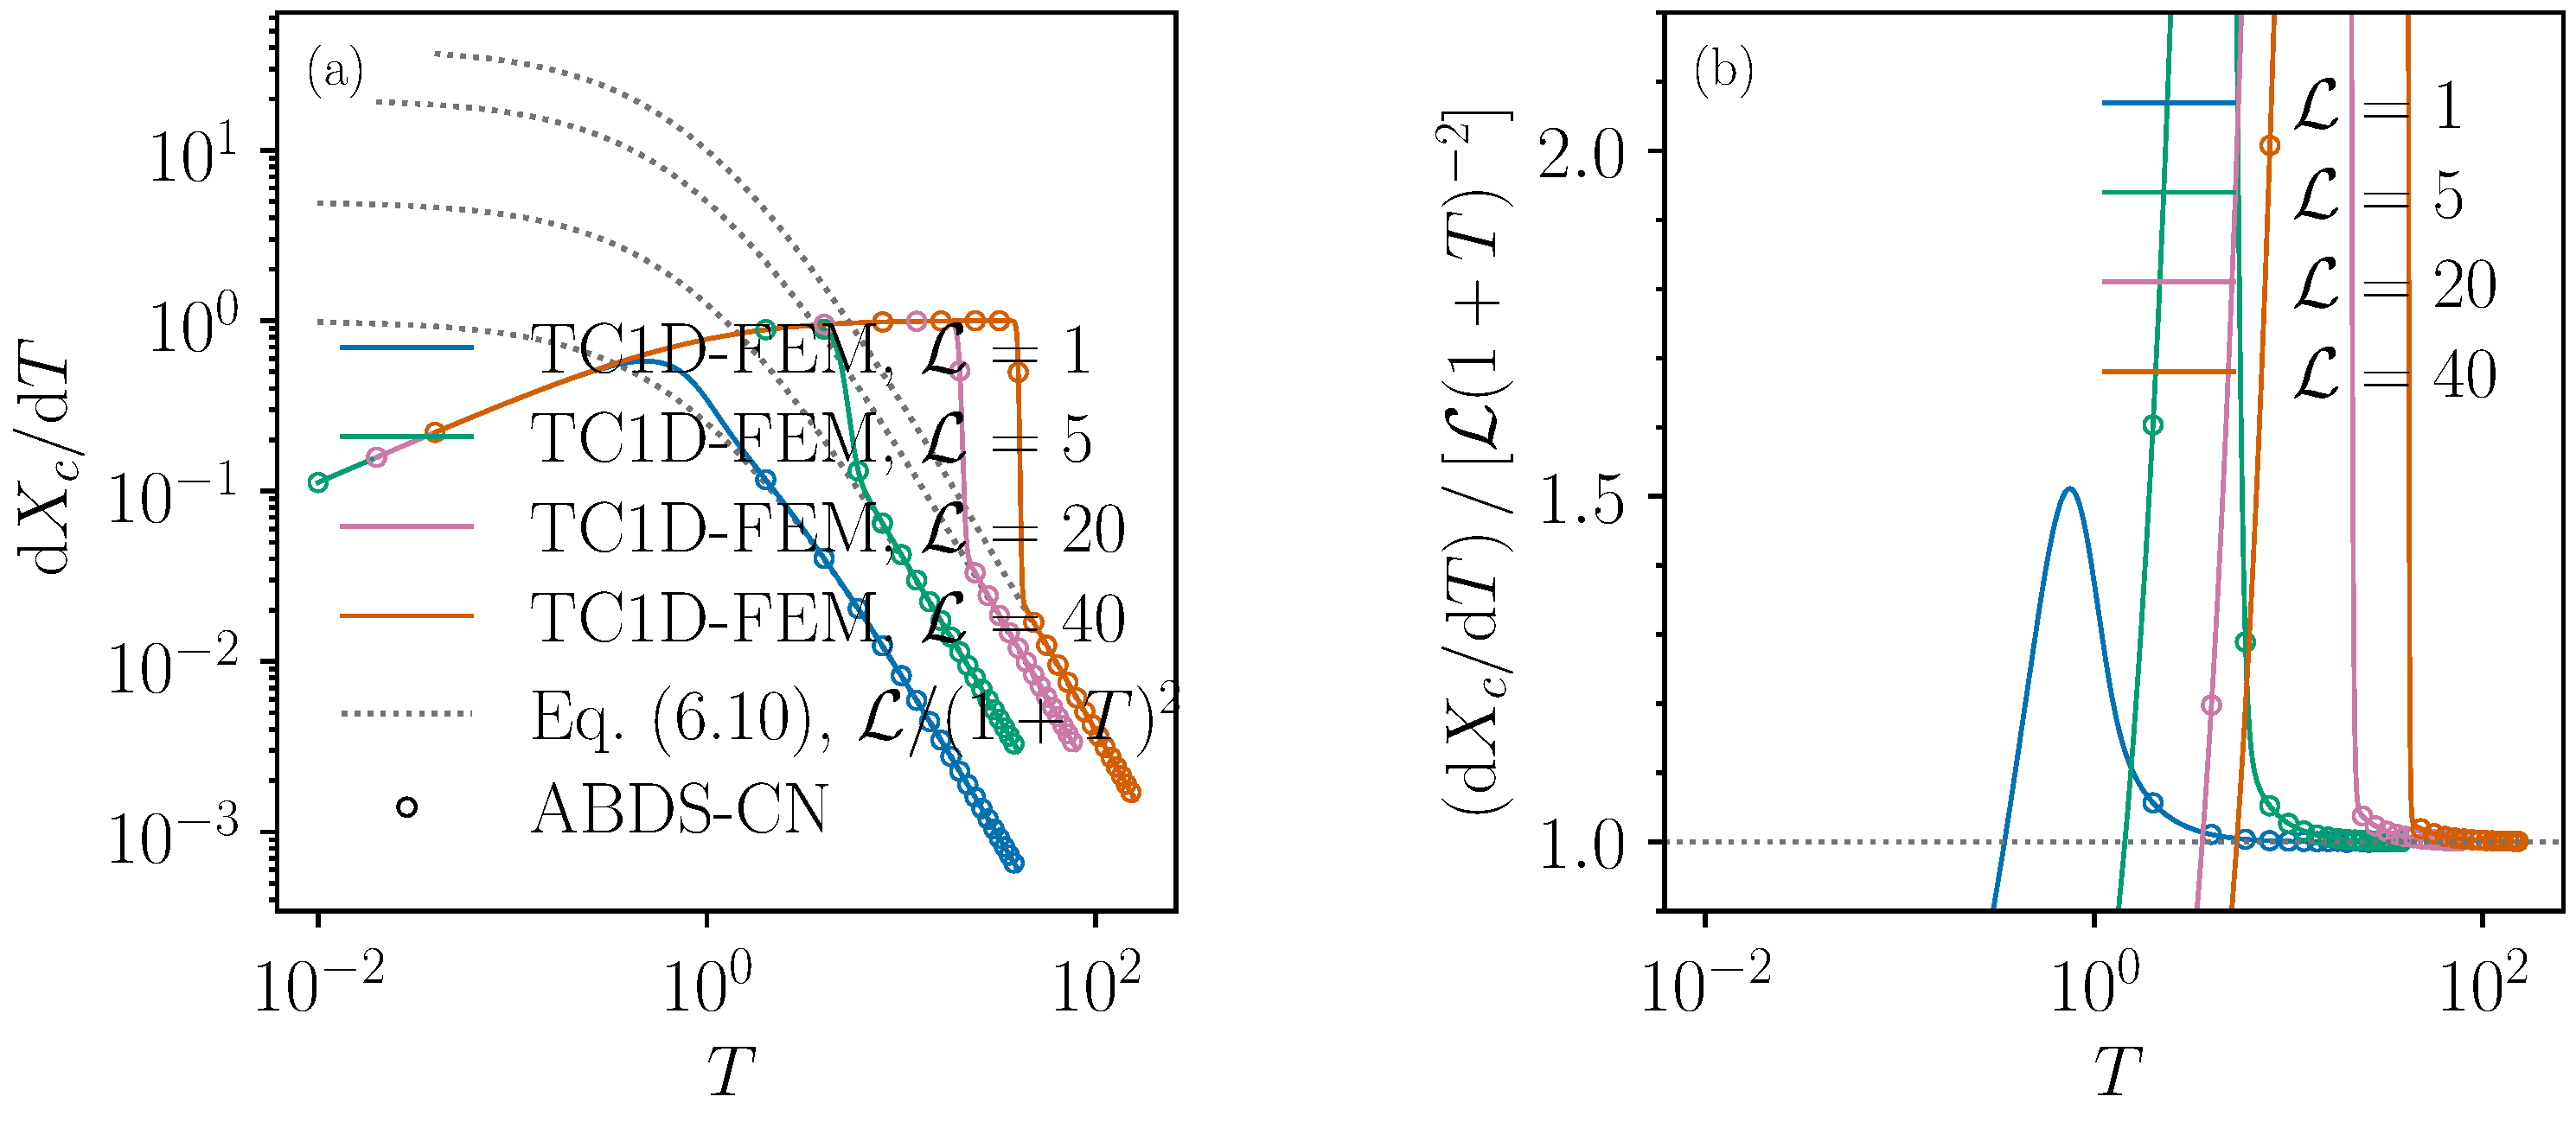
\includegraphics[width=\textwidth]{figures/fig2_deceleration.pdf}
  \caption{Deceleration at finite $\mathcal{L}$. Solid: \TC. Open symbols:
  \AB. Dotted: $\mathcal{L}(1+T)^{-2}$.}
  \label{fig:decel}
\end{figure}

The prediction is reproduced without any adjustable constant. At the end of
each run the ratio of the computed speed to eq.~(6.10) lies between
$1.00002$ and $1.0010$, and the remaining sheet length $\mathcal{L}-\Xc$ agrees
with $\mathcal{L}/(1+T)$ to $1.3\times 10^{-4}$. Continuing the $\mathcal{L}=5$ case to
$T = 400$ shows the relative departure decaying as $O(T^{-2})$, which is the
order of the neglected terms.

\section{Late time at large length}
\label{sec:late}

The regime of principal interest here is $\mathcal{L} \gg T \gg 1$, in which the
edge has reached the Taylor--Culick speed but has not yet sensed the far end.
The reference work gives, for an infinite sheet,
%
\begin{equation}
  \frac{\mathrm{d}\Xc}{\mathrm{d}T} \sim 1 - \frac{1}{(1+T)^{2}} .
  \label{eq:711}
\end{equation}
%
Two points are worth stating before the comparison. The deficit is
$(1+T)^{-2}$, not a pure power $T^{-2}$; fitting a power law in $T$ and
comparing exponents is therefore not a test of eq.~\eqref{eq:711}. And the
coefficient is described in that work as a numerical fit, with the
corresponding expansion coefficient stated to remain undetermined by the
asymptotic analysis and to depend on the history of the retraction.

\subsection{The measured deficit}

Figure~\ref{fig:lateV} shows the speed and the deficit $1-\mathrm{d}\Xc/\mathrm{d}T$.
Forming the ratio $(1+T)^{2}\bigl(1-\mathrm{d}\Xc/\mathrm{d}T\bigr)$, which
eq.~\eqref{eq:711} requires to approach unity, both solvers give

\begin{center}
\begin{tabular}{lccccc}
\toprule
$T$ & $10$ & $20$ & $30$ & $40$ & $50$ \\
\midrule
\AB\ (Richardson $\Delta X \to 0$) & 1.4391 & 1.4891 & 1.4959 & 1.4978 & 1.4985 \\
\TC\ ($\mathcal{L}=200$)           & 1.4382 & 1.4889 & 1.4959 & 1.4977 & 1.4986 \\
\TC\ ($\delta t/2$)                & 1.4382 & 1.4889 & 1.4959 & 1.4977 & 1.4986 \\
\TC\ (mesh $\times 2$)             & 1.4383 & 1.4889 & 1.4960 & 1.4978 & 1.4986 \\
\bottomrule
\end{tabular}
\end{center}

The ratio approaches $3/2$. Extrapolating the plateau with several fit forms
gives $1.5006$, $1.5053$ and $1.4977$, from which we take
%
\begin{equation}
  -U_{-2} = 1.500 \pm 0.003 ,
  \label{eq:threehalves}
\end{equation}
%
consistent with exactly $3/2$ and inconsistent with unity.

\begin{figure}[htbp]
  \centering
  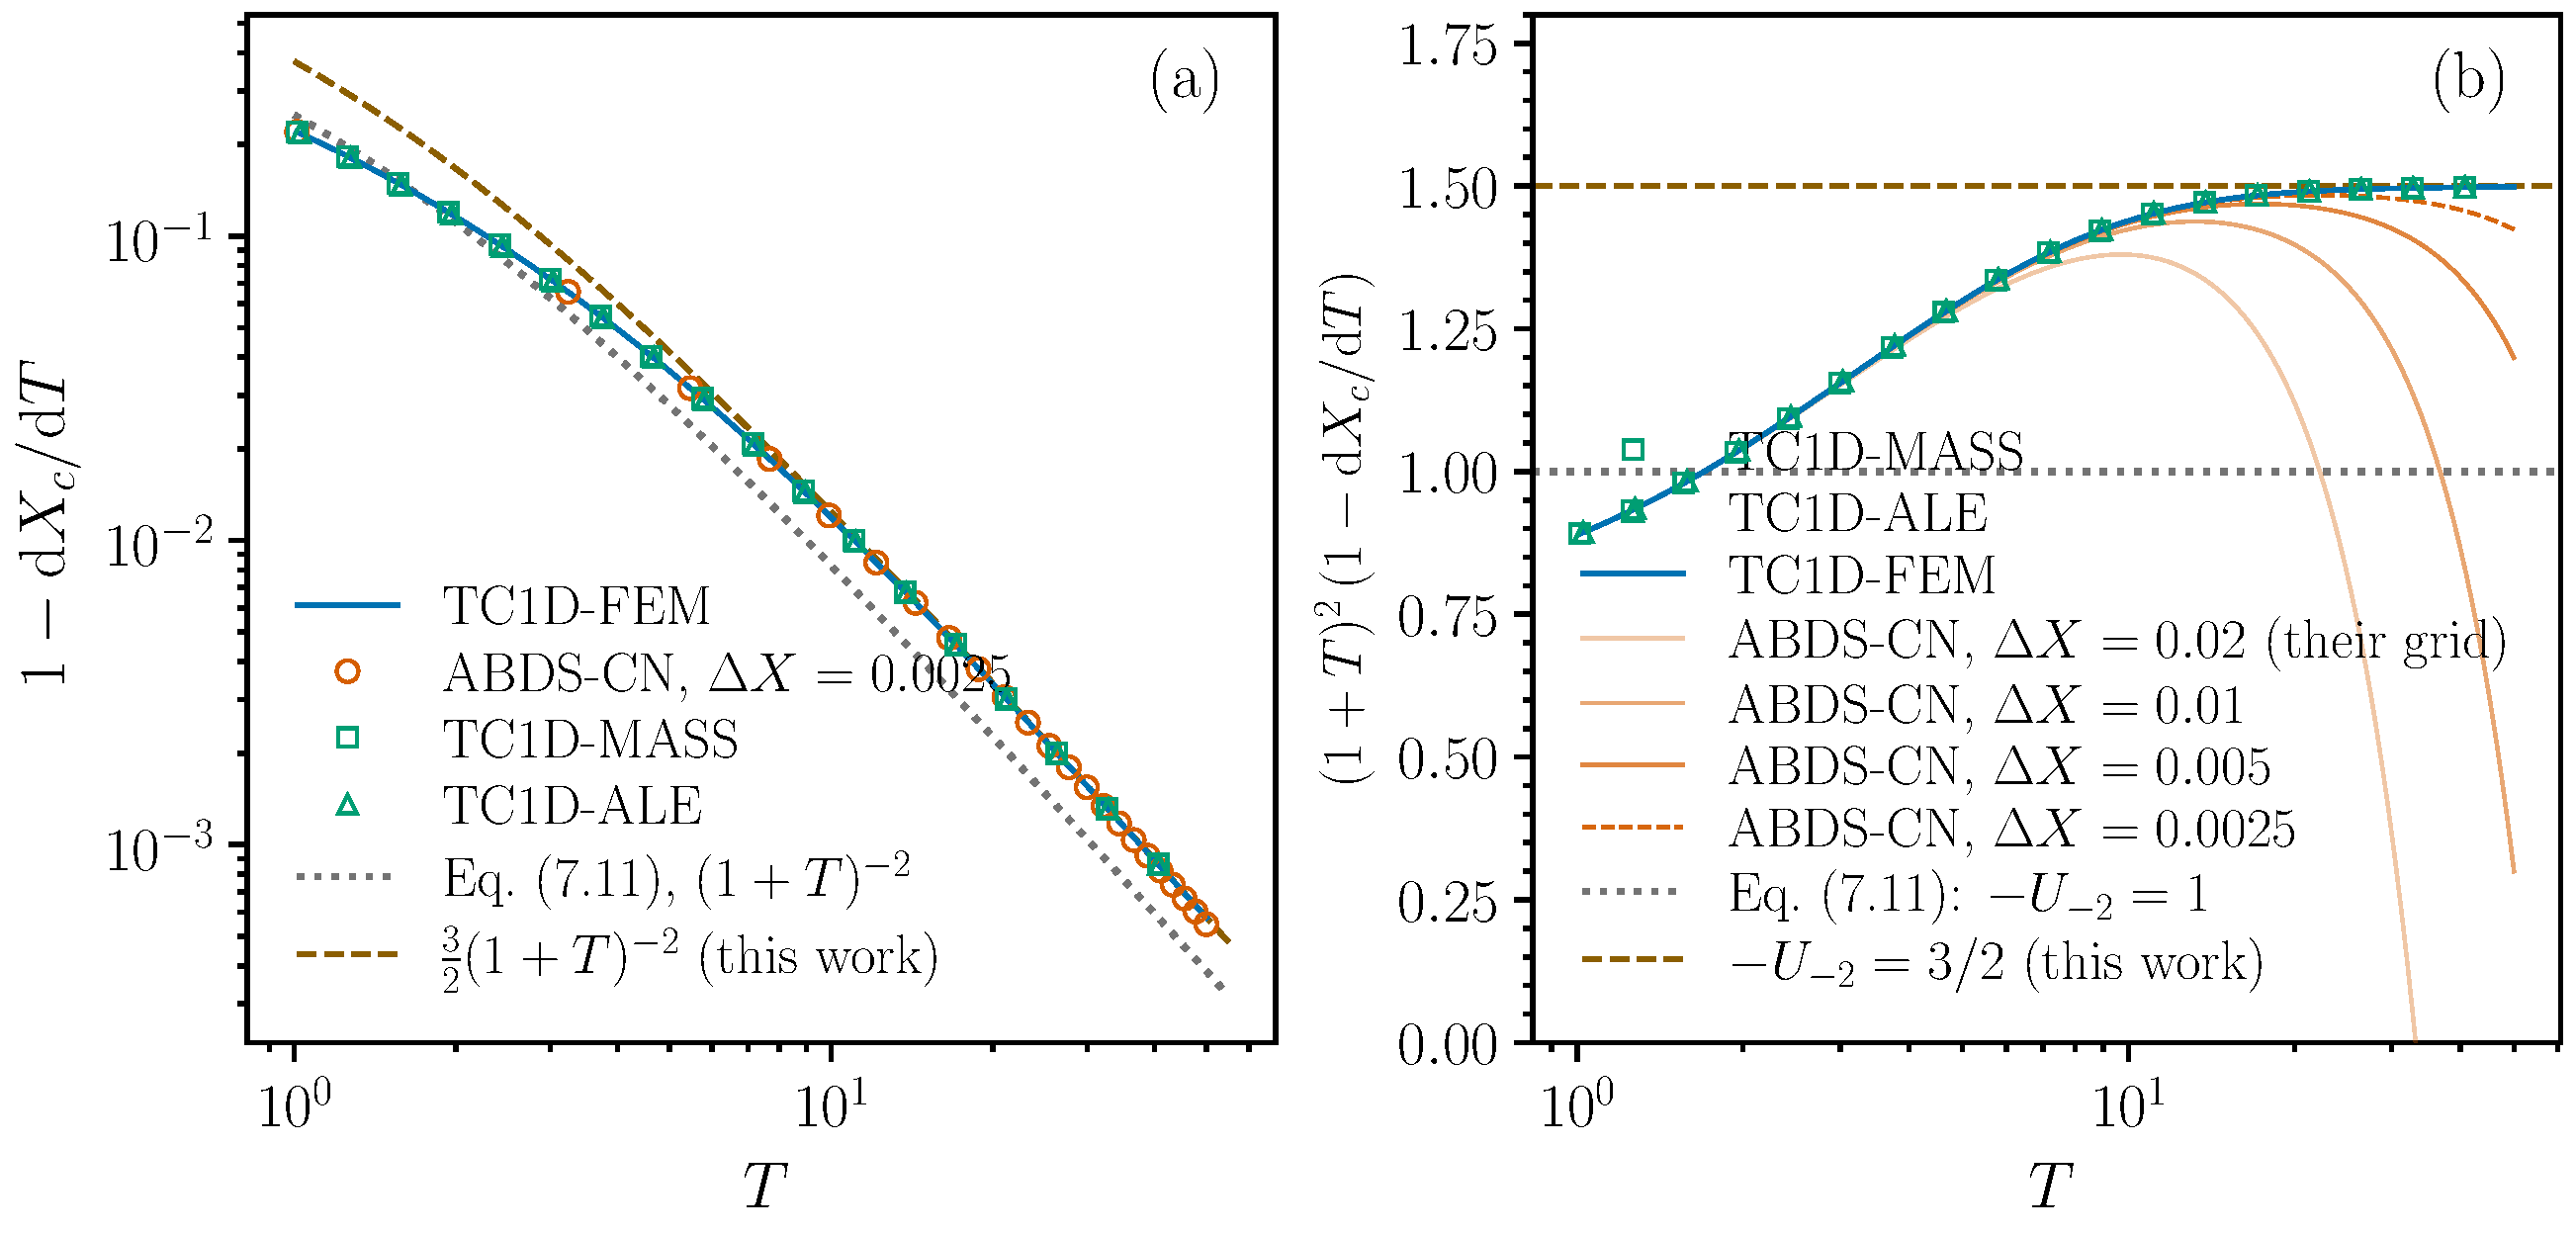
\includegraphics[width=\textwidth]{figures/fig3_latetime_V.pdf}
  \caption{Late-time speed and deficit at large $\mathcal{L}$. Solid: \TC.
  Open symbols: \AB. Dotted: eq.~\eqref{eq:711}.}
  \label{fig:lateV}
\end{figure}

The result is insensitive to every numerical parameter varied: halving the
timestep changes it by $1.3\times 10^{-8}$ and doubling the mesh by $1.6\times 10^{-6}$,
against a deficit of $5.8\times 10^{-4}$ at $T=50$. \AB\ converges at an observed
order of $2.000$--$2.002$ in $\Delta X$, and its Richardson limit agrees with
\TC\ to $4.8\times 10^{-5}$.

A second, independent check supports the same conclusion. The reference work's
eq.~(7.17) gives $\Xc \sim T+1$, whereas its own eqs.~(7.8) and~(7.10),
its eqs.~(7.13) and~(7.16), and direct integration of eq.~\eqref{eq:711} all
give $\Xc \sim T-1$. Both solvers measure $\Xc(50) - 50 = -0.971$. The
relation $\Xc \sim T - 1$ is equivalent to the exact statement
$\int_0^{\infty}\bigl(1 - \mathrm{d}\Xc/\mathrm{d}T\bigr)\,\mathrm{d}T = 1$.

\subsection{A two-term form}

A form consistent with the measured coefficient and with the integral
constraint is
%
\begin{equation}
  \frac{\mathrm{d}\Xc}{\mathrm{d}T} \simeq
  1 - \frac{3}{2}\frac{1}{(1+T)^{2}} + \frac{1}{(1+T)^{3}} ,
  \label{eq:twoterm}
\end{equation}
%
which reproduces the numerics to within 2.7\% for $T \ge 5$,
against 33\% for eq.~\eqref{eq:711} over the same range. We
emphasise that eq.~\eqref{eq:twoterm} is constructed to match a measured
coefficient and an exact constraint; it is not derived.

\subsection{Profiles and the tip thickness}

Figure~\ref{fig:profiles} compares thickness and velocity profiles against the
reference work's eqs.~(7.13) and~(7.14). The tip-thickness relation
$H(\Xc,T) = 1+T$ is reproduced to a maximum relative deviation of $3.6\times 10^{-5}$
over $1 \le T \le 50$. The profile predictions agree to 0.043\%
and 1.55\% respectively at $T=50$, improving monotonically with
$T$.

\begin{figure}[htbp]
  \centering
  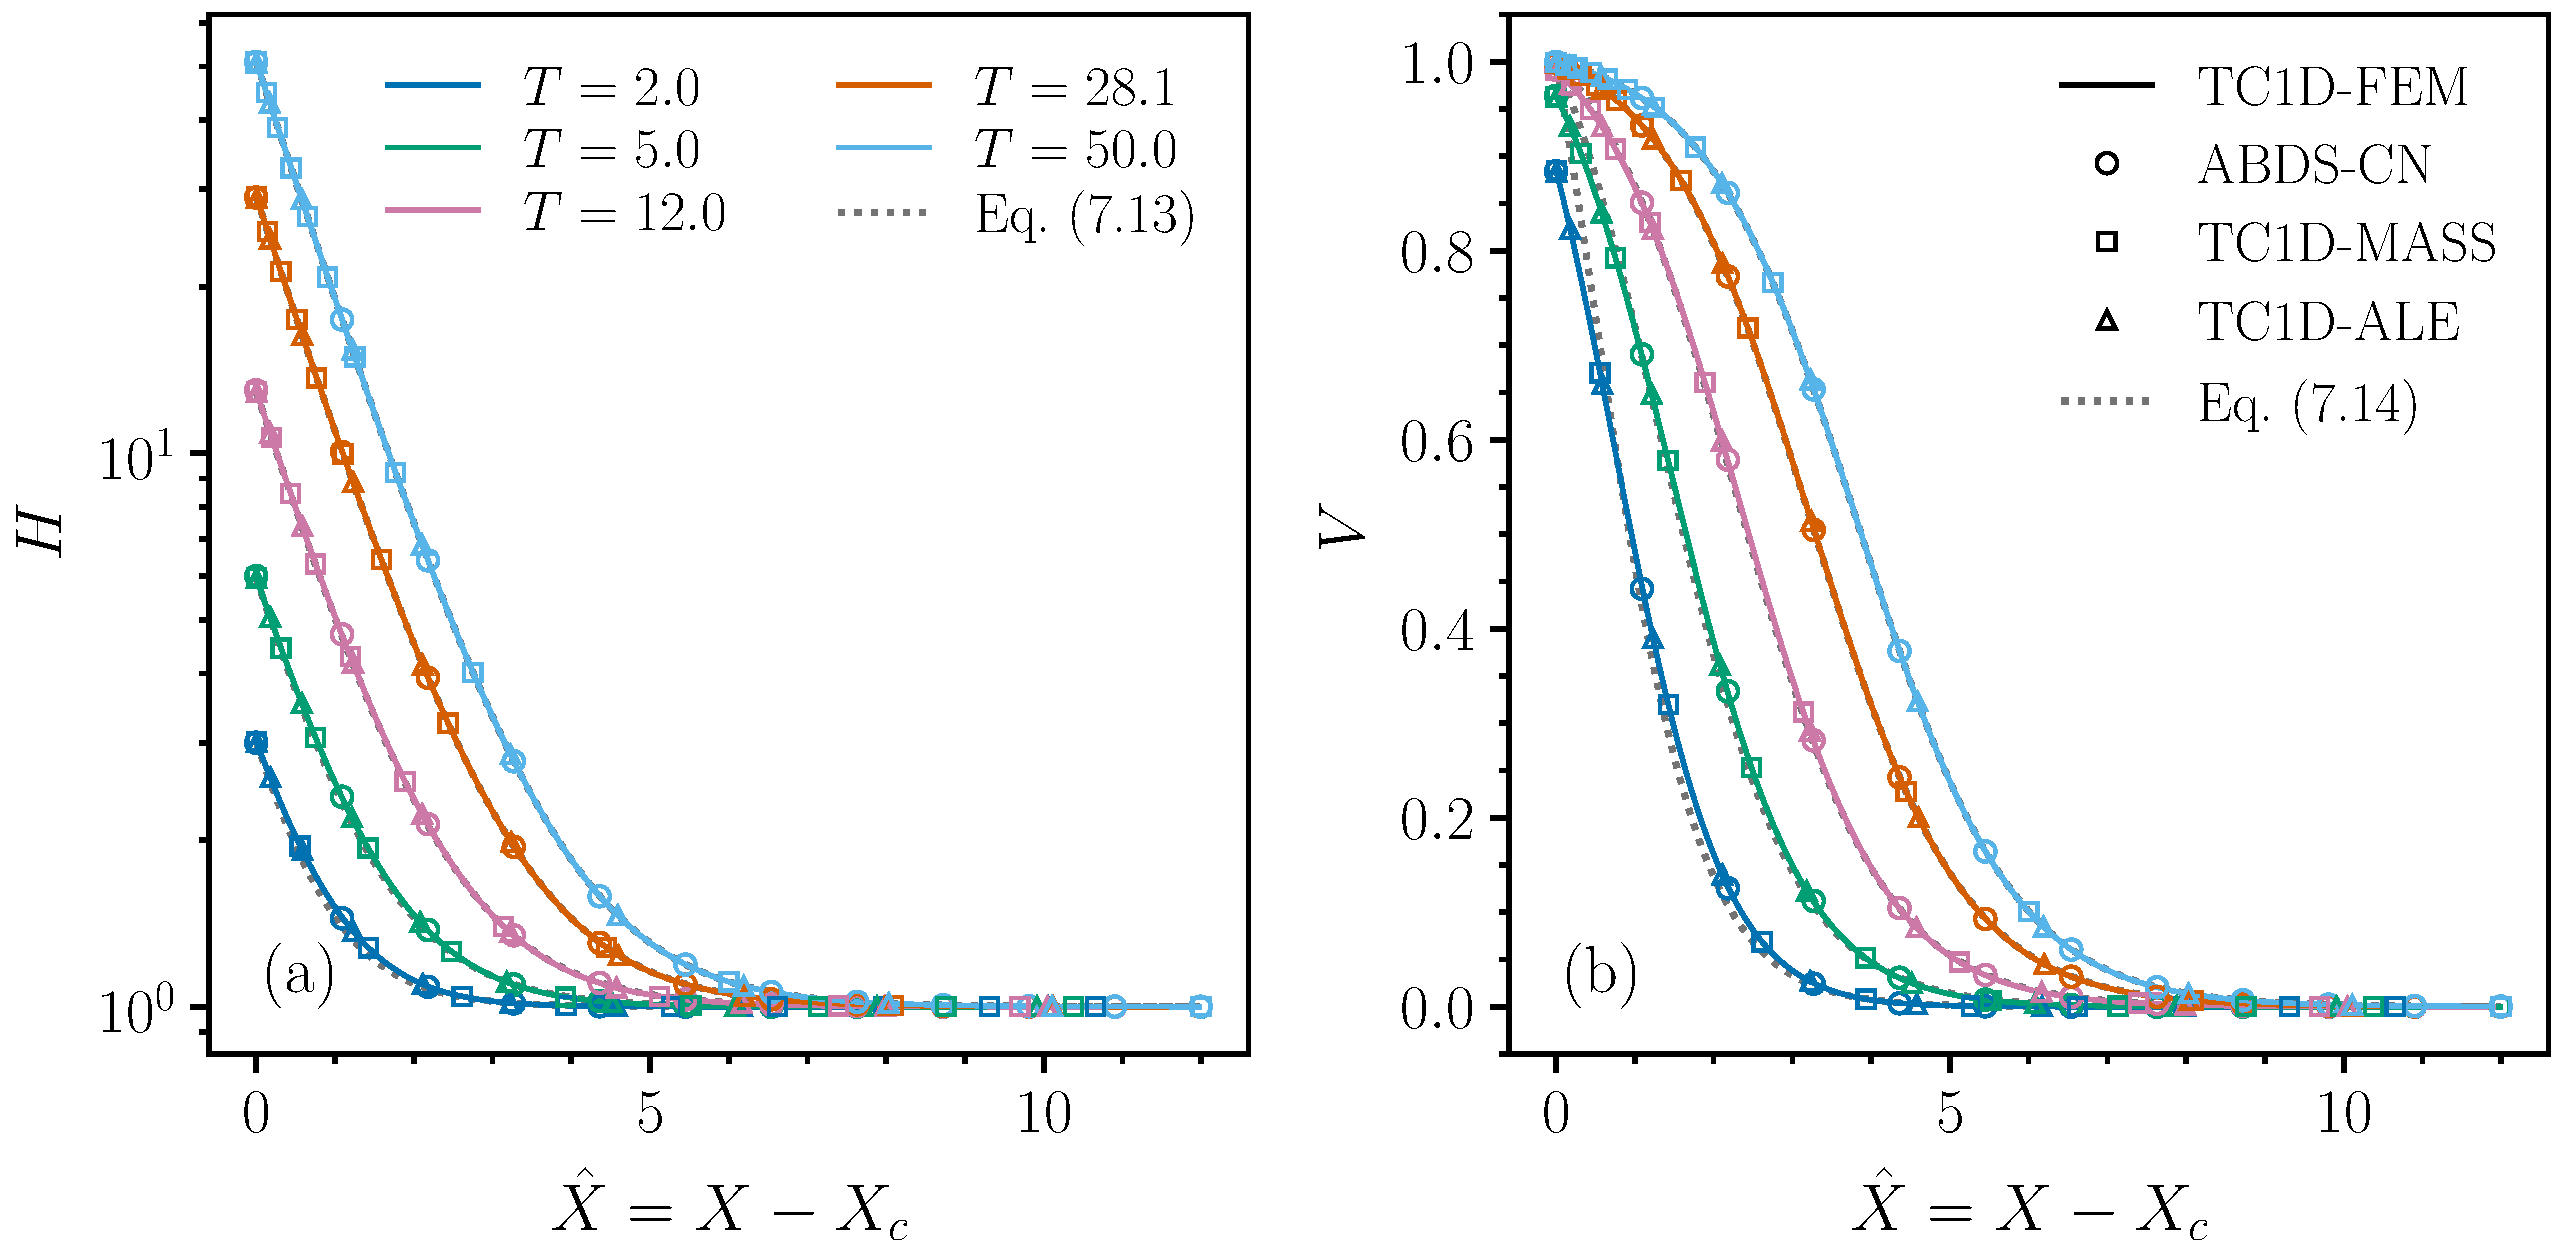
\includegraphics[width=\textwidth]{figures/fig3_latetime_profiles.pdf}
  \caption{Thickness and velocity profiles at large $\mathcal{L}$. Solid: \TC.
  Open symbols: \AB. Dotted: eqs.~(7.13) and~(7.14).}
  \label{fig:profiles}
\end{figure}

\section{The crossover time}
\label{sec:tc}

For large $\mathcal{L}$ the edge decelerates from the Taylor--Culick speed onto
the finite-sheet law of \S\ref{sec:decel}. The reference work reports the
crossover time $\Tc$ and its duration $\Delta \Tc$ as functions of
$\mathcal{L}$, with $\Tc = \mathcal{L}$ for large $\mathcal{L}$.

Neither quantity is defined in closed form in that work, so an operational
definition is adopted here and applied identically to both solvers; it is
stated with the figure. Figure~\ref{fig:tc} compares both solvers against
values digitised from the published figure.

\begin{figure}[htbp]
  \centering
  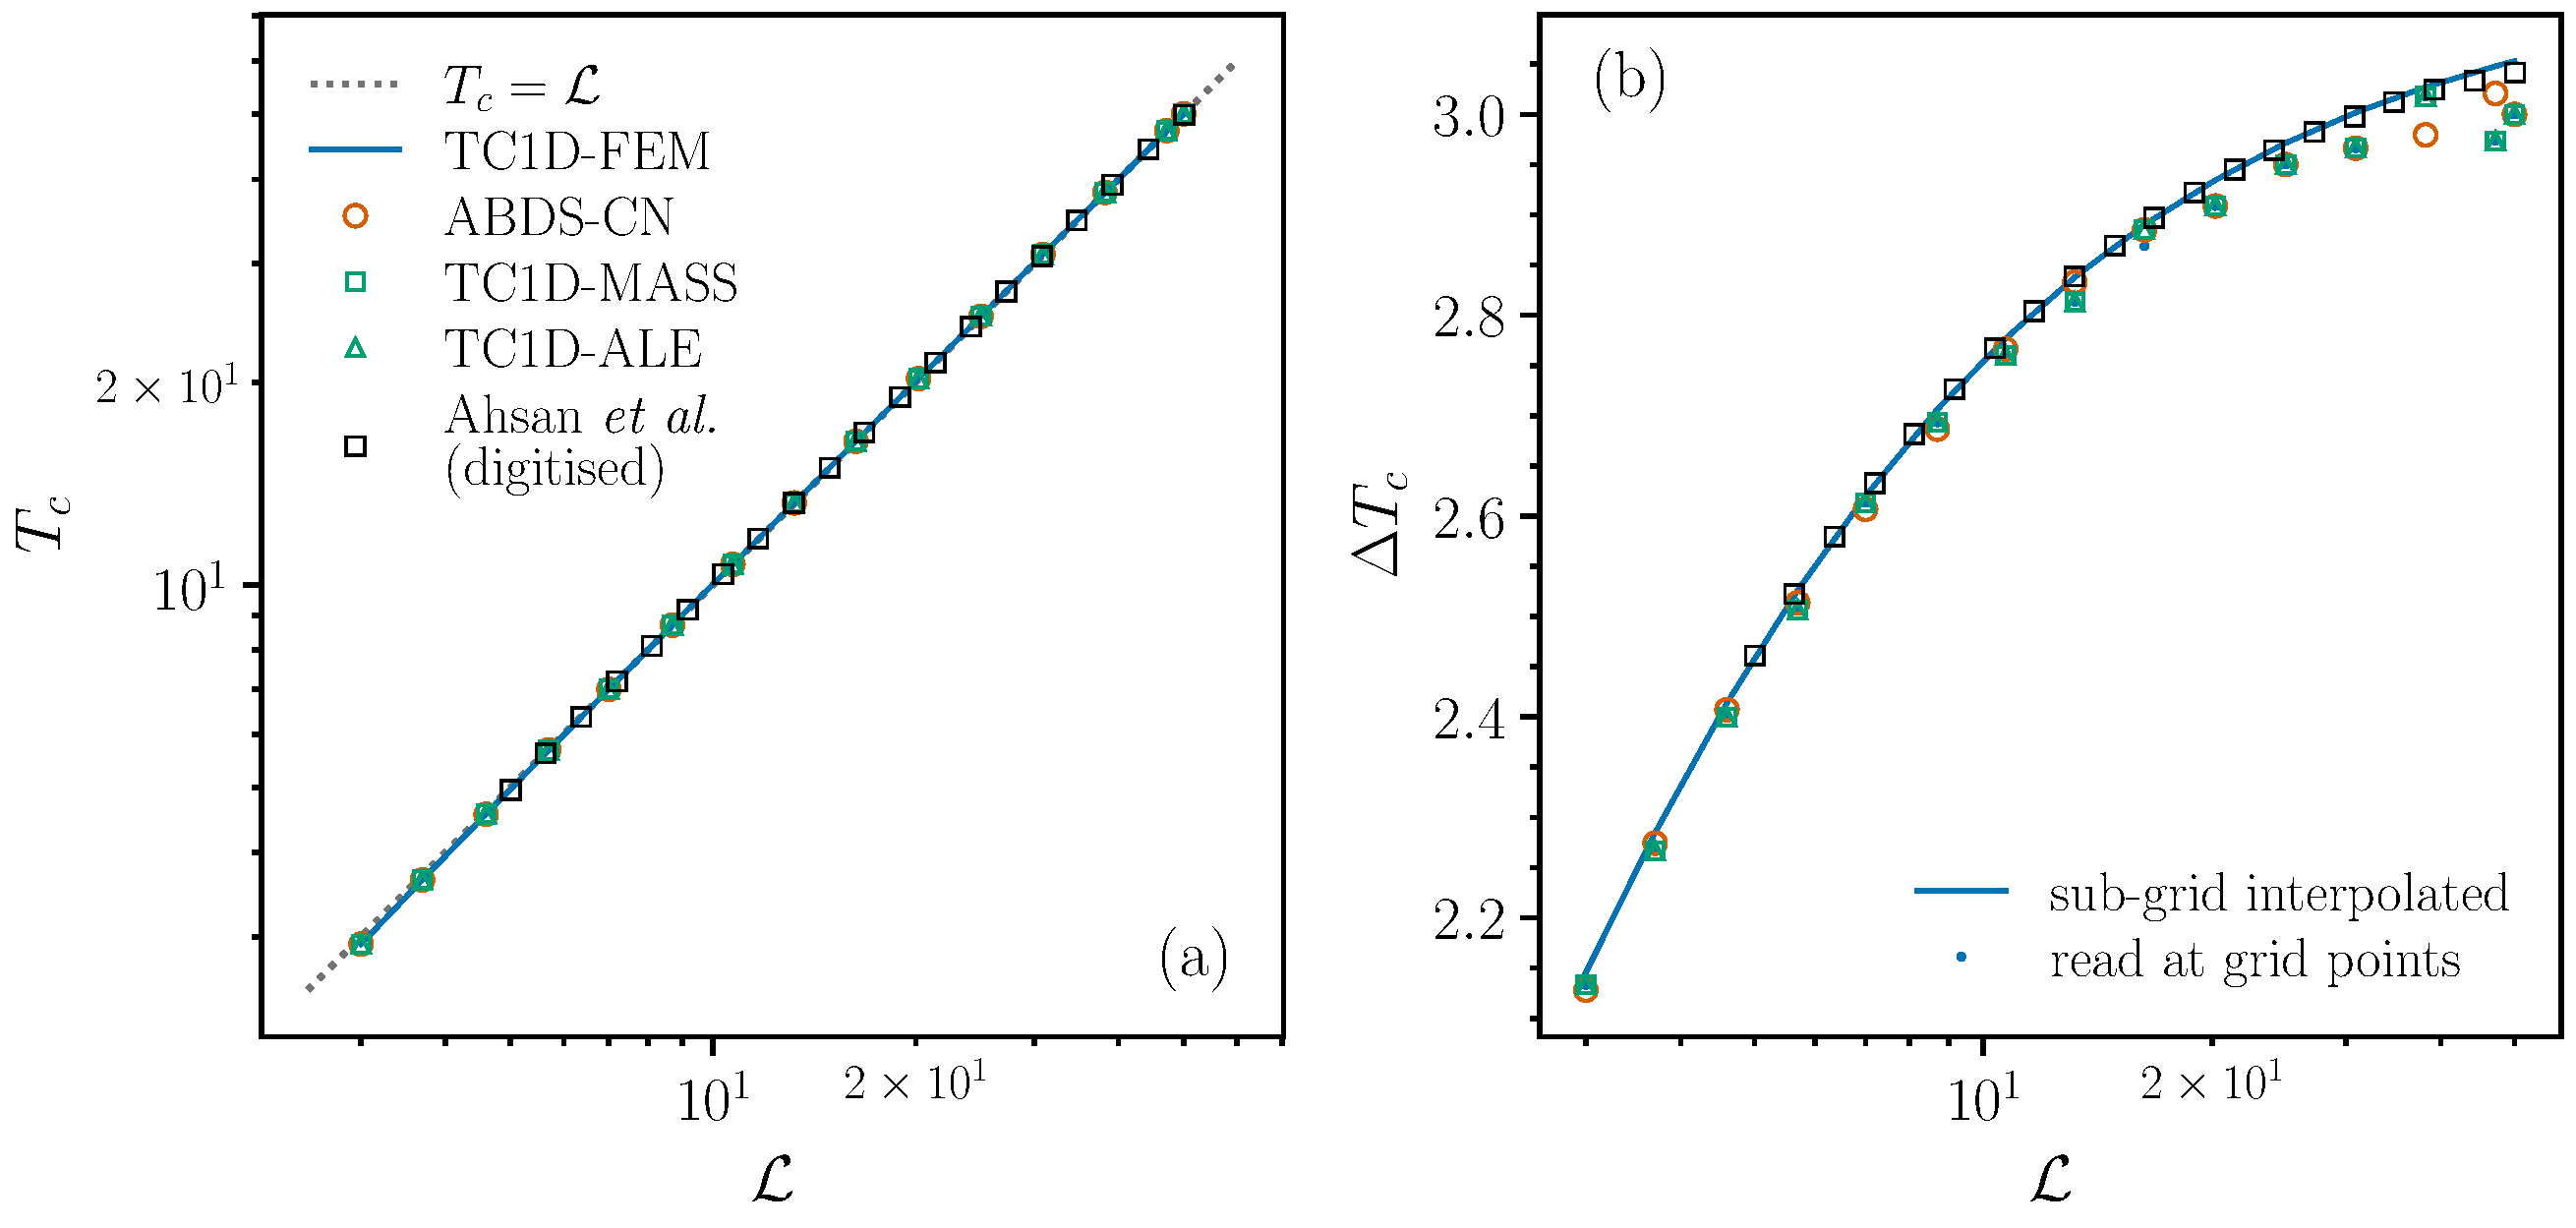
\includegraphics[width=\textwidth]{figures/fig4_Tc_vs_L.pdf}
  \caption{Crossover time $\Tc$ and duration $\Delta \Tc$ against
  $\mathcal{L}$. Solid: \TC. Open symbols: \AB. Circles: values digitised from
  the published figure.}
  \label{fig:tc}
\end{figure}

We find $\Tc/\mathcal{L} = 1$ to within 0.25\% for
$\mathcal{L} \ge 7$. Against the digitised values, $\Tc$ agrees to
0.142\% RMS, within the estimated digitisation uncertainty of
0.2\%, and $\Delta \Tc$ to $0.024$ absolute
(1.5\%).

One point of definition should be recorded. The text of the reference work
describes $\Delta \Tc$ as a full width at half maximum, while the released code
computes twice that width. The published values are consistent with the code.
Both conventions are reported here.

\appendix

\section{Fidelity of the reference transcription}
\label{sec:port}

\AB\ is a transcription of released \textsc{Matlab} into Python. To establish
that the transcription is faithful rather than merely plausible, the original
code was executed under GNU Octave and compared with the transcription at
identical parameters. Over six configurations the largest absolute difference
in the retraction speed is $5.0\times 10^{-10}$, and the largest normalised difference
across all twenty-four recorded quantities is $3.0\times 10^{-8}$. The former is the
resolution at which the original code writes its output, so the two agree to
every digit that can be compared.

\begin{figure}[htbp]
  \centering
  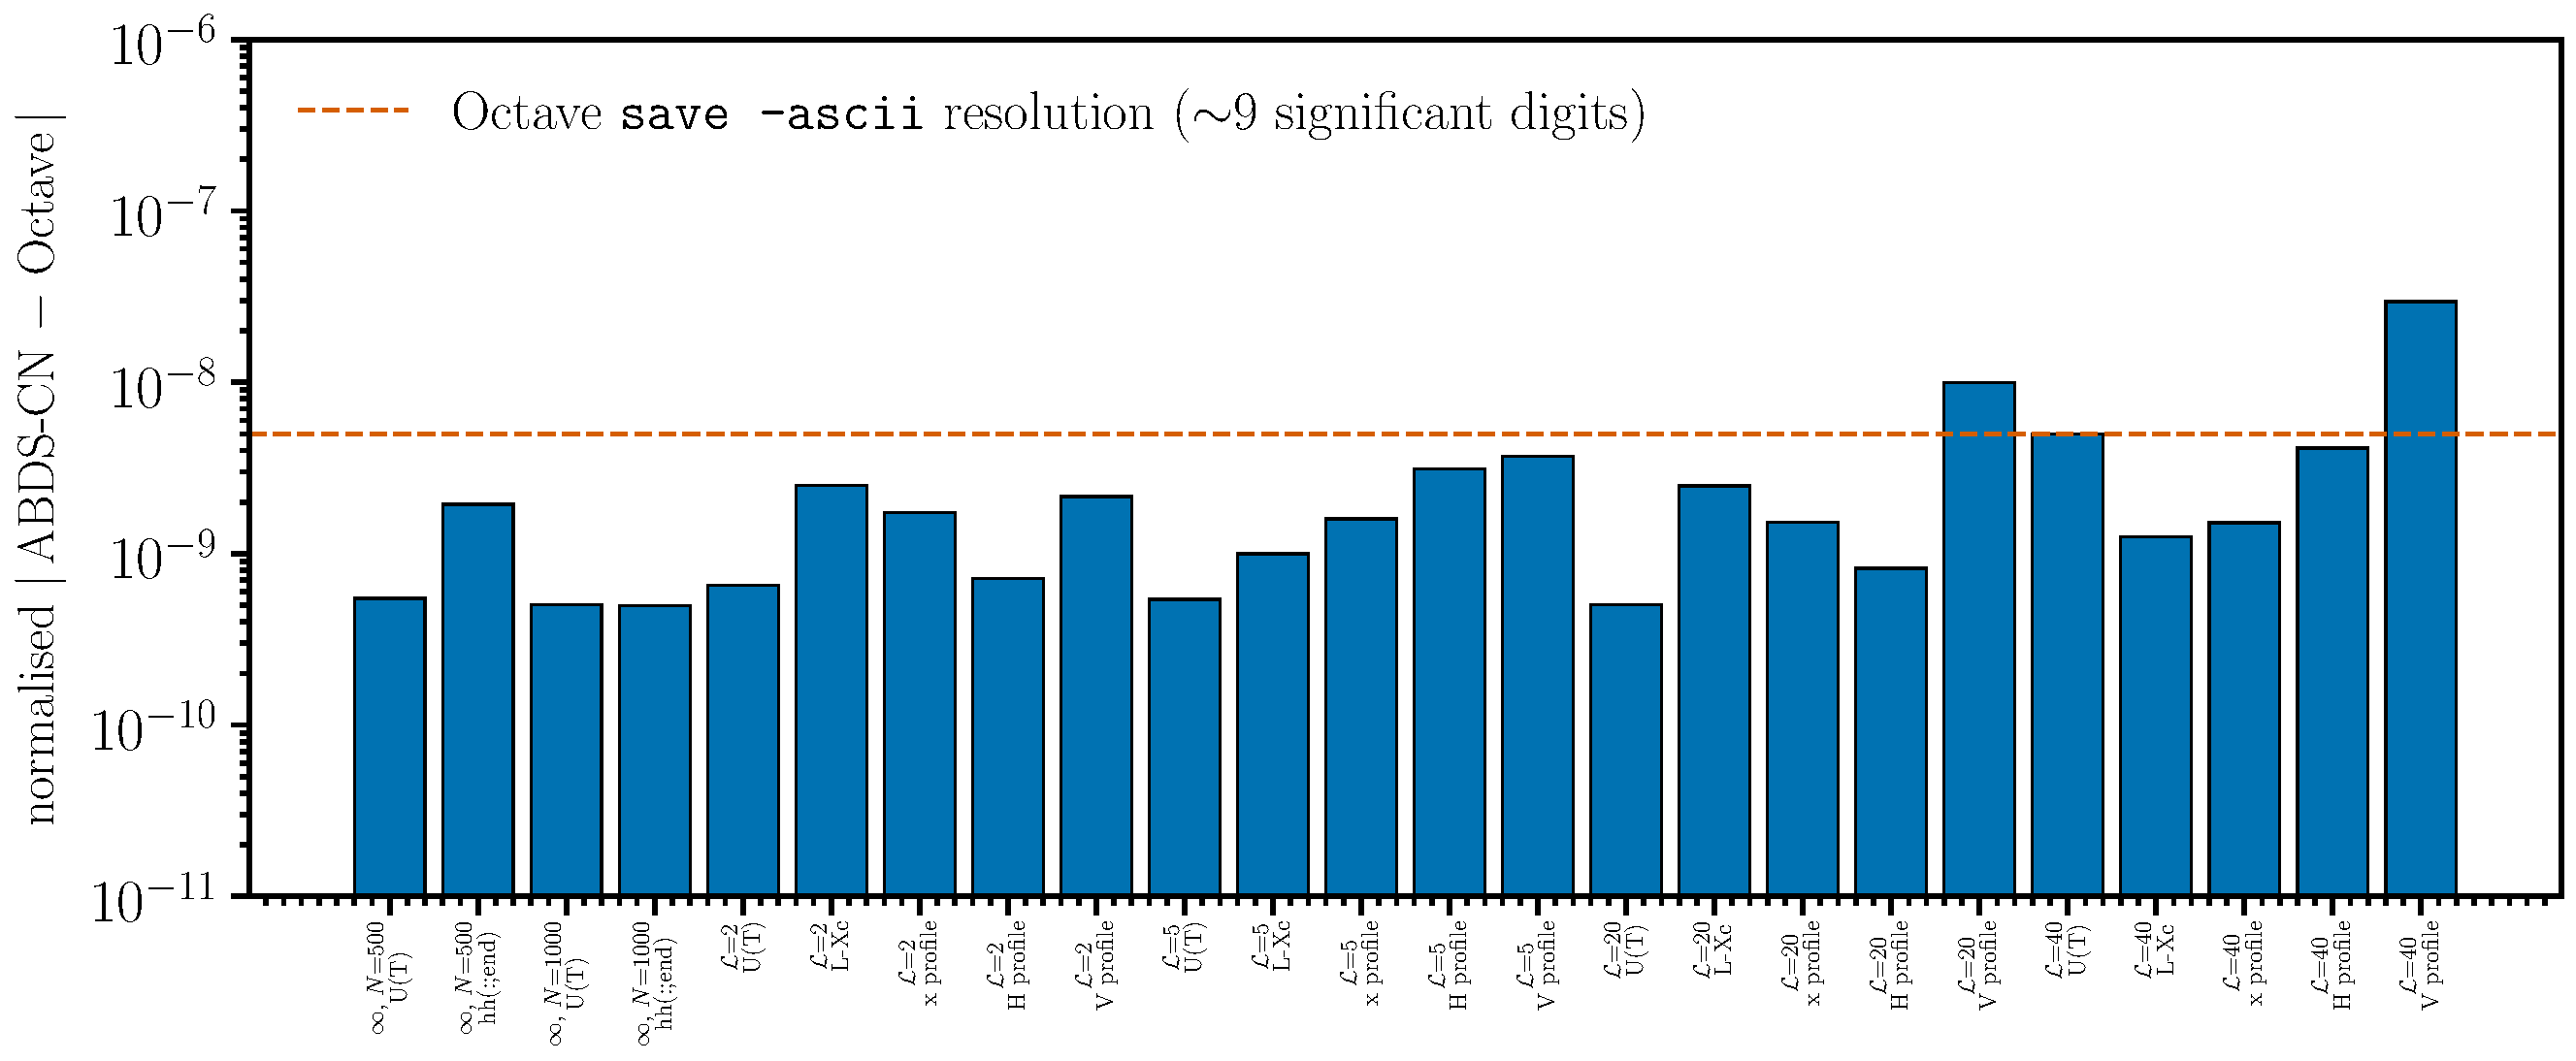
\includegraphics[width=\textwidth]{figures/figA1_port_fidelity.pdf}
  \caption{Original released code executed under GNU Octave, against the Python
  transcription \AB, at several $\mathcal{L}$.}
  \label{fig:port}
\end{figure}

\section{Reproduction}

The campaign comprises 72 cases. Each is recorded in a manifest with its
parameters and the exact command that regenerates it, alongside the derived
series used for every figure and table in this document.

\end{document}
